\section{Results: the nine-dimension measurement map}
\label{sec:results}

On the harmonized FACE V0 baseline ($N=9{,}013$), the hybrid bifactor/ESEM yields a \textbf{nine-dimension
transdiagnostic map}: a general factor $G$ (functional burden) plus eight specific axes ---
cognition, metabolic, inflammatory, sleep, developmental-risk, suicidality, mania, and substance
(Table~\ref{tab:map}). Five are continuous-anchored (marginalized: cognition, metabolic, inflammatory, sleep,
mania); three carry non-Gaussian indicators through explicit latents (suicidality, developmental, substance)
alongside $G$. Every coordinate is estimated from observed cells only, with no imputation.

\begin{table}[h]\centering\small\sffamily
\caption{The reported transdiagnostic map. Loadings are posterior means; suicidality's binary ISF items are on
the logit scale. $|\lambda_G|$ is the mean absolute bifactor loading on $G$ --- the \emph{severity
entanglement} of each domain (\S\ref{sub:bioperpG} refines biology's value under the correlated-$G$
identification).}
\label{tab:map}
\begin{tabular}{L{3.2cm} L{6.4cm} R{2.0cm} R{1.6cm}}
\toprule
\hdr{dimension} & \hdr{anchored by} & \hdr{primary $\lambda$} & \hdr{$|\lambda_G|$}\\
\midrule
\rowcolor{facebg} $G$ --- functional burden & FAST 0.90, EGF 0.73, EQ-5D, CGI-S (functioning + severity only; no symptom content) & --- (general) & ---\\
cognition & CVLT, WAIS coding/digit-span, fluency, TMT-B & 0.57 & 0.27\\
\rowcolor{facebg} metabolic & BMI, waist, BP, glucose, HbA1c, lipids & 0.32 & 0.08\\
inflammatory & CRP, WBC, neutrophils, platelets, eosinophils & 0.39 & 0.07\\
\rowcolor{facebg} sleep & PSQI objective sub-scores, ESS & 0.48 & 0.25\\
developmental-risk & CTQ, age-of-onset, WURS, perinatal, family history & 0.42 & 0.12\\
\rowcolor{facebg} suicidality & ISF binary ideation/attempt $+$ count & 2.2--2.7 (logit) & 0.3--0.6\\
mania & YMRS 0.57, Altman 0.76 (BP) & 0.49--0.76 & 0.15\\
\rowcolor{facebg} substance & alcohol/cannabis lifetime SUD, nicotine & 0.38--0.69 (logit) & 0.13\\
\bottomrule
\end{tabular}
\end{table}

\subsection{The empirical atlas, beside the theory}
The scientific deliverable of the measurement map is the \emph{prior $\to$ posterior} comparison
(Figure~\ref{fig:priorposterior}): the theory map of where instruments were \emph{expected} to load, placed
beside the fitted map of where they \emph{actually} load. Reading the two together is the whole story --- the
block-diagonal primary structure is recovered, the faint $G$ column appears over the functioning anchors only,
the windows land on $G$, and the biology candidate resolves into two distinct blocks. The posterior atlas alone
is the per-indicator loading fingerprint of the map (Figure~\ref{fig:empatlas}).

\begin{figure}[p]\centering
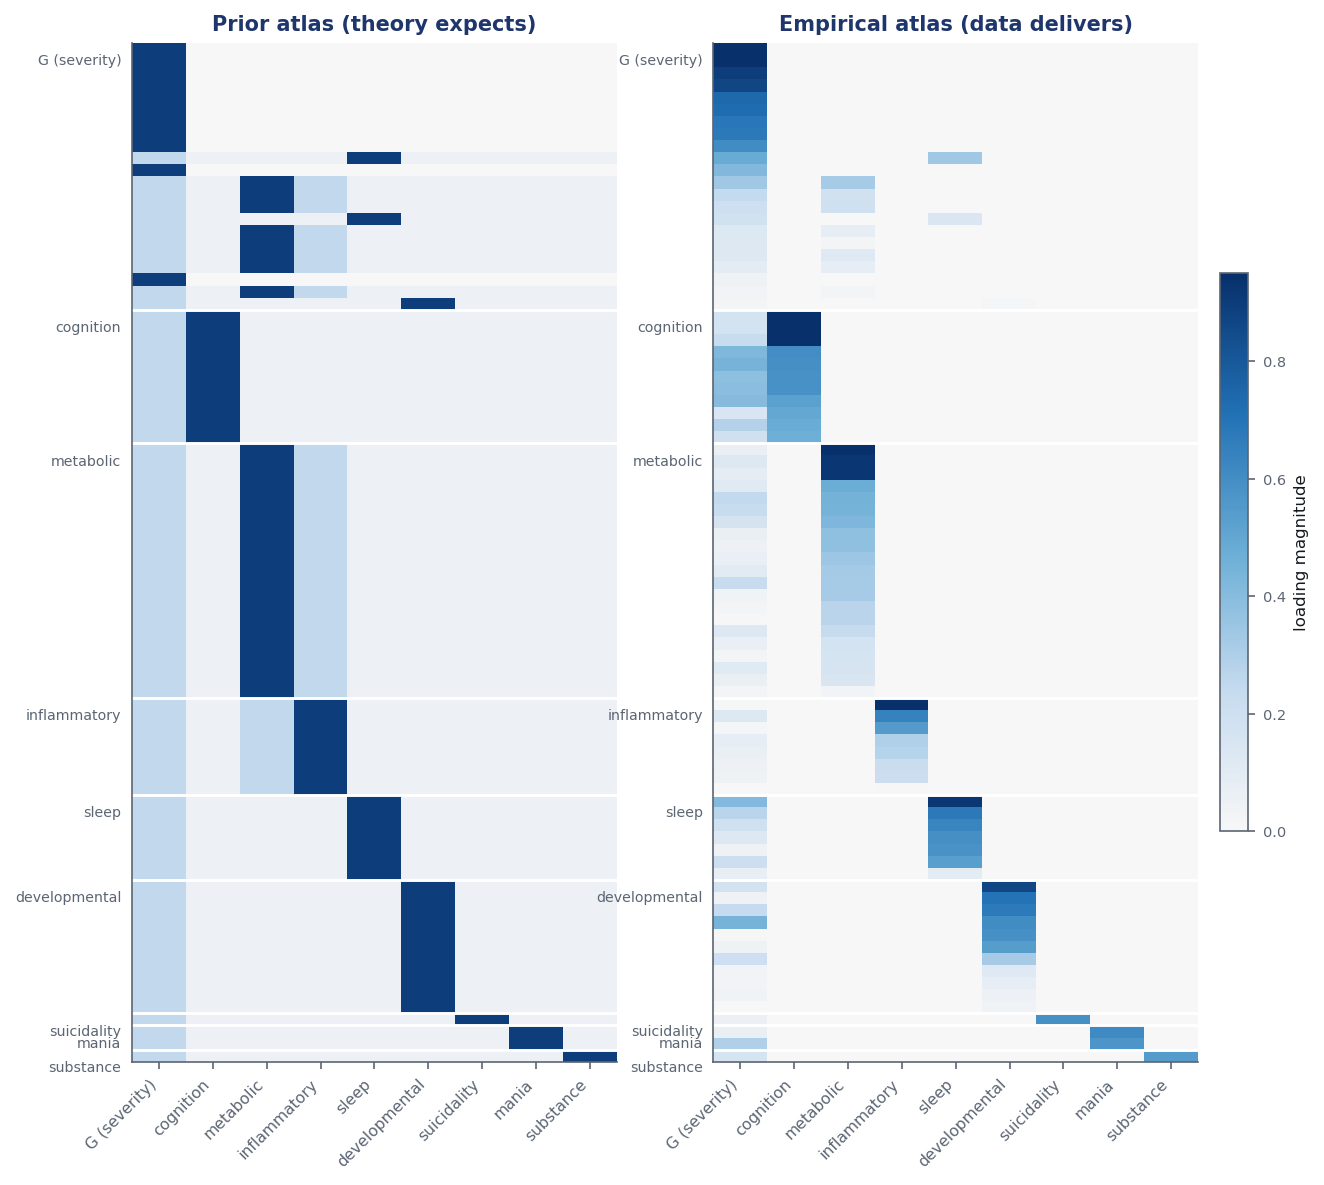
\includegraphics[width=\linewidth,height=0.88\textheight,keepaspectratio]{figures/fig_prior_posterior.png}
\caption{Prior $\to$ posterior. \emph{Left:} the soft-prior atlas (theory --- where each instrument is
\emph{expected} to load). \emph{Right:} the fitted posterior atlas (data --- where it \emph{actually} loads).
Rows are the modelled indicators grouped by home factor, in a shared order; columns are the nine dimensions.
The data recover the block-diagonal primaries theory proposed, add a faint general-factor column over the
functioning anchors, and --- crucially --- earn structure theory only hypothesised (the metabolic/inflammatory
split). This side-by-side is the hybrid model adjusting theory with evidence.}
\label{fig:priorposterior}
\end{figure}

\begin{figure}[h]\centering
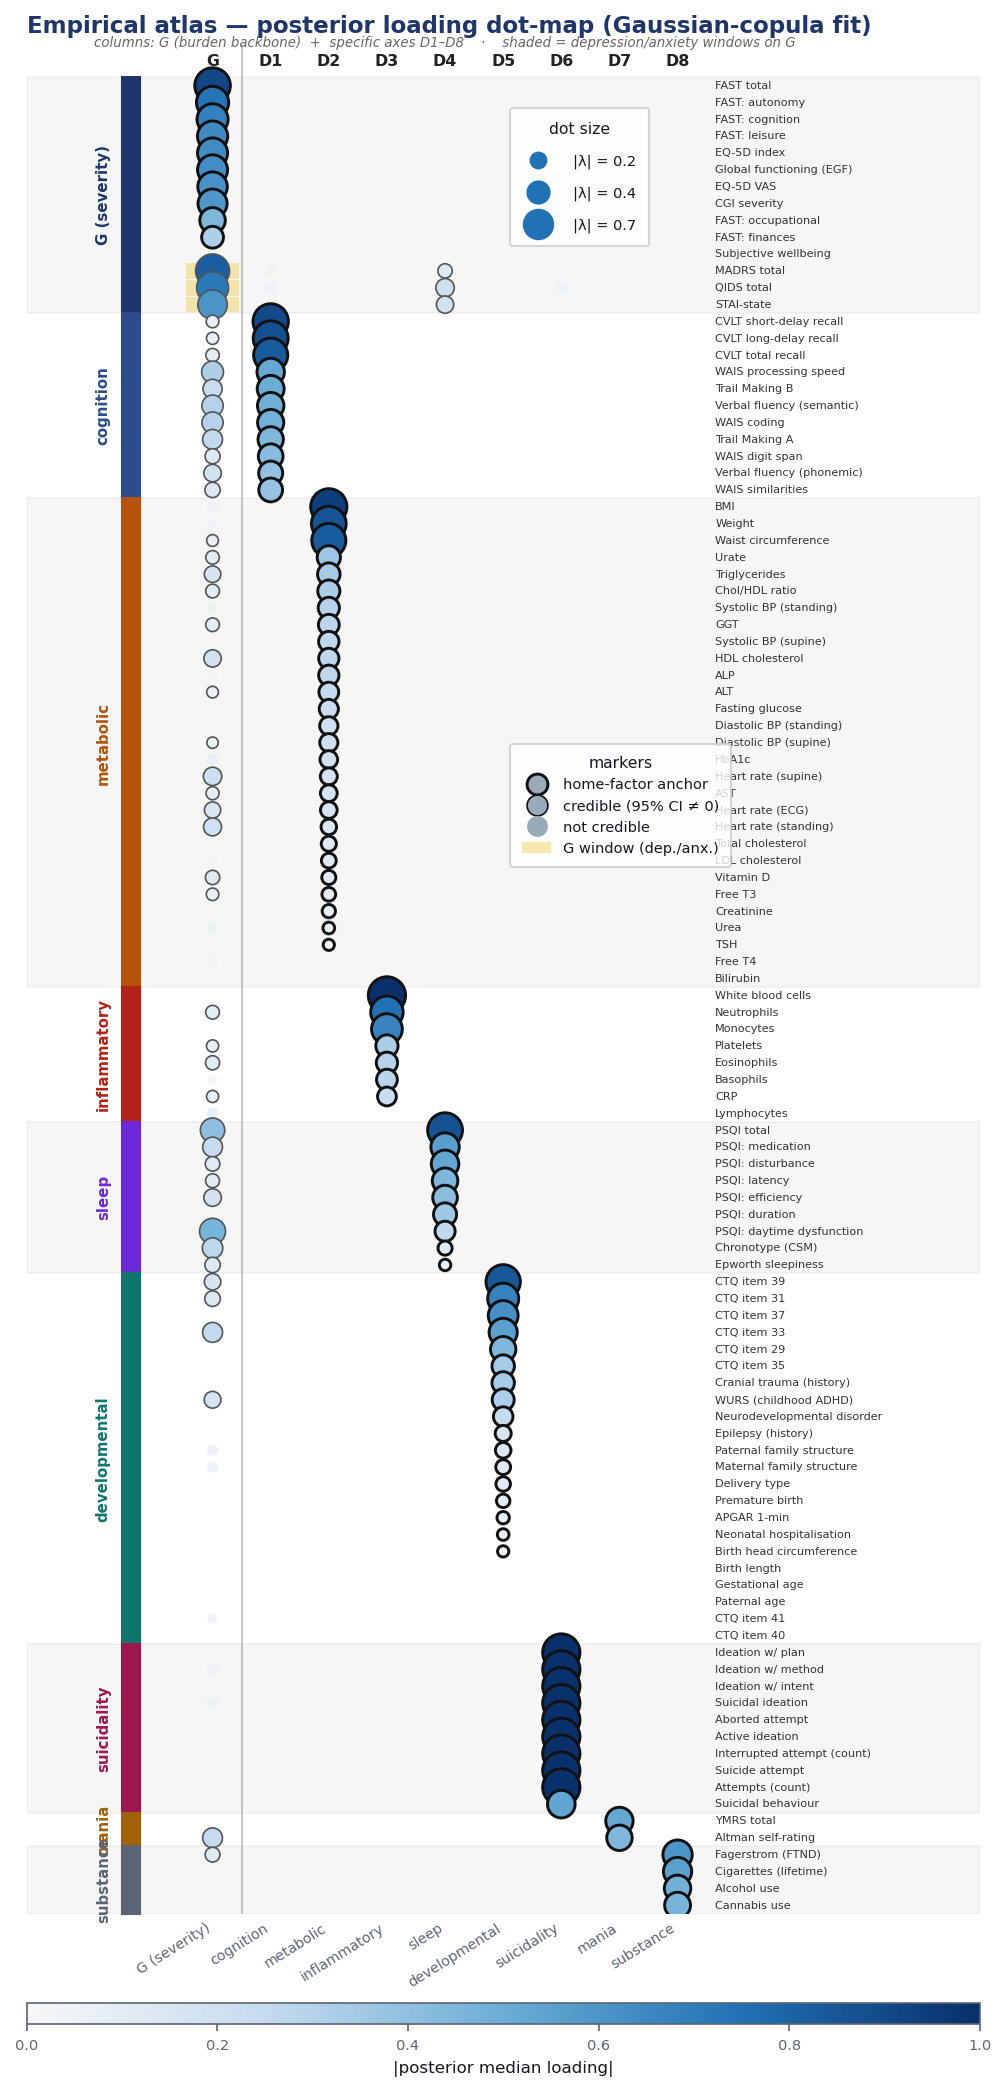
\includegraphics[width=0.64\linewidth]{figures/fig_empirical_atlas.png}
\caption{The empirical atlas --- posterior loading magnitudes, rows grouped by home factor. Each dimension is
anchored by its own block; the leftmost ($G$) column is faint for the specific items (biology faintest of all)
and dark only for the functioning anchors at the top.}
\label{fig:empatlas}
\end{figure}

\subsection{The headline: biology is the least severity-entangled domain}
\label{sub:bioperpG}
\certified\ The load-bearing finding concerns how much each specific axis is entangled with overall illness
burden $G$. Because the strict bifactor constraint ($G\perp$ specifics) could in principle \emph{understate}
that entanglement, it is tested under the correlated-$G$ sensitivity arm, which \emph{frees} $G$ to correlate
with the specifics (Figure~\ref{fig:biologyg}).

\begin{figure}[h]\centering
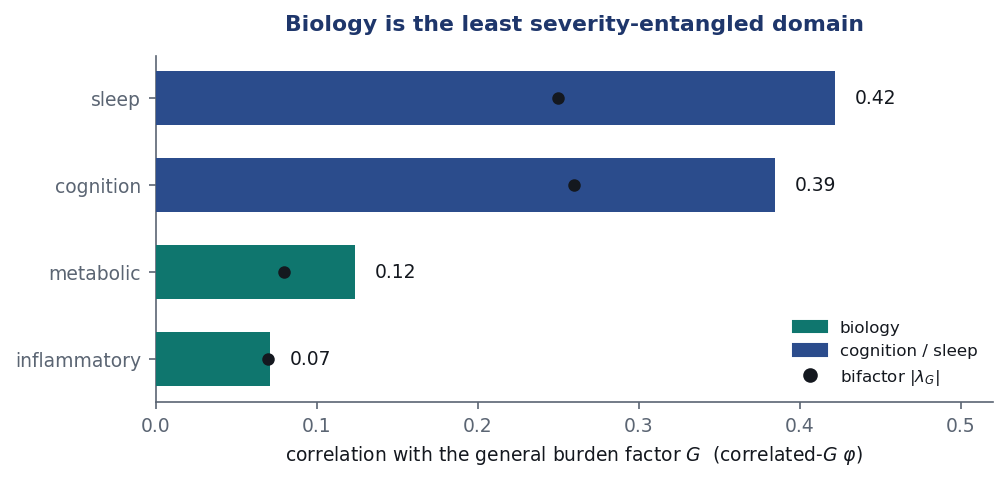
\includegraphics[width=0.80\linewidth]{figures/fig_biology_g.png}
\caption{Severity entanglement per domain. Bars: the correlated-$G$ factor correlation with $G$; dots: the
stricter bifactor direct loading $|\lambda_G|$ (the two agree on the ordering). Metabolic ($0.12$) and
inflammatory ($0.07$) burden are nearly independent of $G$, far below cognition ($0.39$) and sleep ($0.42$).
Mania and substance are likewise low ($|\lambda_G|$ $0.15$ and $0.13$).}
\label{fig:biologyg}
\end{figure}

\begin{keyresult}[Biology rides on axes severity does not see]
Freeing $G$ to correlate with the specifics, it correlates $+0.07$ with inflammatory and $+0.12$ with
metabolic, versus $+0.39$ with cognition and $+0.42$ with sleep. So metabolic and inflammatory load carry
$98.5$--$99.5\%$ of their variance \emph{independent} of how impaired a patient is overall. Two patients
who look equally ill on a clinician's global impression can differ sharply in biological load --- precisely the
severity-independent signal a biology-aware stratification can exploit. \emph{(The clean continuous-backbone
estimate, metabolic$\sim$$G$ $0.12$, supersedes an earlier provisional mixed-fit read of $0.28$; both
agree biology is least entangled --- an honest downward correction the dual-identification test exists to
produce.)}
\end{keyresult}

The conservative reading of $G$ itself supports this. $G$ is anchored \emph{only} by functioning and
global-severity items (FAST $0.90$, EGF $0.73$) and carries \emph{no} symptom content --- a patient's
subjective-illness rating loads $\approx 0$. $G$ is therefore a transdiagnostic \emph{impairment} axis, not a
latent ``p-factor'' liability to psychopathology --- a deliberately modest interpretation that avoids the
bifactor over-claim.

\subsection{Distinct axes, and depression as a window}
\documented\ The dimensions are \emph{weakly} correlated --- mean $|\Phi_{\text{off-diagonal}}|\approx 0.10$
(Figure~\ref{fig:phi}). The map carries genuine multidimensional information, not one severity factor in
disguise. The only non-trivial couplings are clinically coherent: metabolic$\leftrightarrow$inflammatory
$0.19$ (an immunometabolic link --- the two are related but \emph{not} collinear, vindicating the split),
suicidality$\leftrightarrow$developmental $0.23$ (childhood adversity $\to$ suicidality), and
sleep$\leftrightarrow$developmental $0.19$.

\begin{figure}[h]\centering
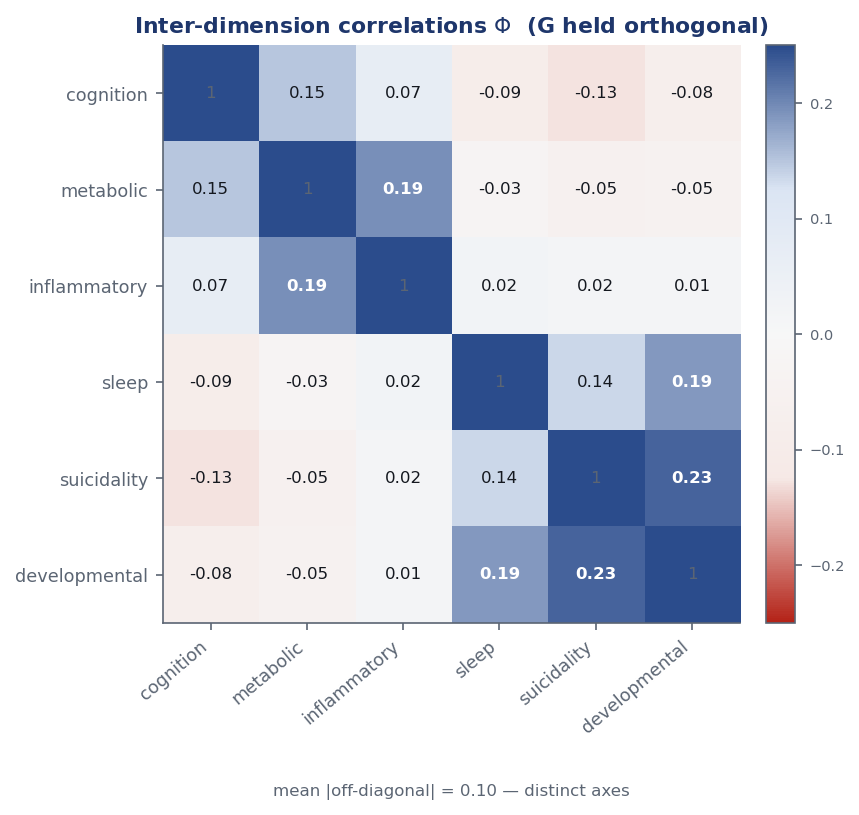
\includegraphics[width=0.56\linewidth]{figures/fig_phi_heatmap.png}
\caption{Inter-dimension correlations $\Phi$ (specific block; $G$ orthogonal by construction). The off-diagonal
is weak (mean $0.10$); the strongest links --- metabolic$\leftrightarrow$inflammatory and
suicidality$\leftrightarrow$developmental --- are exactly the clinically expected ones. mania and substance
integrate under the same $\Phi$ with low couplings (cross-seed Tucker $\varphi$ $0.993$).}
\label{fig:phi}
\end{figure}

The composite depression/anxiety instruments are \emph{not} a separate dimension: MADRS, QIDS, and STAI load
$0.80$, $0.77$, and $0.66$ on $G$ (with minor sleep side-loadings), behaving as cross-loading \emph{windows}
onto overall burden. Depression and anxiety severity are expressions of functional burden here, not a separable
affective latent --- the model was free to grow an eleventh factor and declined.

\subsection{The map is larger than seven: mania and substance}
Two candidates had indicators but were initially \emph{deferred} from the staged build. Closing that gap
\textbf{confirmed both as real, low-$G$ axes} and the joint nine-dimension model was re-fit rather than
bolted on. \textbf{Mania} is anchored by YMRS ($0.57$) and the Altman self-report ($0.76$ in BP), with
$|\lambda_G|$ $0.15$. \textbf{Substance} is anchored by lifetime alcohol/cannabis use-disorder and nicotine
indicators ($+0.38$ to $+0.69$ on the logit scale) under their proper Bernoulli/negative-binomial likelihoods,
with $|\lambda_G|$ $0.13$. Manic activation and substance use are thus distinct transdiagnostic axes, not
reducible to severity --- and worth carrying into stratification.

\subsection{Suicidality as a mixed-likelihood axis}
\documented\ That non-Gaussian psychopathology composes with the continuous biology in one correlated-factor
space is itself a result. The binary ISF ideation and attempt items load strongly on their own axis
\emph{and} modestly on $G$ (Table~\ref{tab:suic}), with $0$ divergences --- the proper Bernoulli/count
likelihoods integrate into the shared $\Phi$ without breaking identification or being crushed onto a
pseudo-continuous scale.

\begin{table}[h]\centering\small\sffamily
\caption{Suicidality indicators: home loading and bifactor $G$ loading (logit scale). Ideation and attempt
load on the specific axis \emph{and} on overall burden --- clinically coherent.}
\label{tab:suic}
\begin{tabular}{L{4.8cm} R{3.0cm} R{3.0cm}}
\toprule
\hdr{ISF indicator} & \hdr{home (suicidality)} & \hdr{$G$ (bifactor)}\\
\midrule
\rowcolor{facebg} isf01--05 (ideation) & $+2.2$ to $+2.7$ & $+0.33$ to $+0.56$\\
isf08 / isf09 (attempt) & $+1.8$ / $+2.0$ & $+0.12$ / $+0.34$\\
\rowcolor{facebg} isf08a (attempt, ordinal) & $+1.7$ & $+0.12$\\
isf09a (attempt, count) & $+1.6$ & $+0.31$\\
\bottomrule
\end{tabular}
\end{table}

\subsection{What the data rejected, and the verdict on every candidate}
\rejected\ \textbf{Anhedonia} does not form a stable distinct factor. With a single thin BP/DR indicator it is
non-identified ($\widehat{R}=1.54$, $\mathrm{ESS}=7$); when it forms, its indicator loads $0.61$ on $G$ and the
QIDS-total window cross-loads $0.37$ onto it (near-collinear, since the anhedonia anchor is a QIDS component).
Its variance is absorbed by $G$ + the depression windows. This is the anticipated outcome --- a result, not a
failure.

The full adjudication (Table~\ref{tab:adjudication}): of the ten prior-matrix candidates, \textbf{nine are
confirmed} (one a split, one a proxy), \textbf{one rejected} (anhedonia); three pre-matrix constructs are
\code{not_testable}; depression/anxiety are windows. No candidate remains deferred.

\begin{table}[h]\centering\small\sffamily
\caption{Per-candidate adjudication (the empirical dimension atlas, §6). Theory proposed; the FACE data
disposed.}
\label{tab:adjudication}
\begin{tabular}{L{4.6cm} L{3.4cm} L{6.0cm}}
\toprule
\hdr{candidate} & \hdr{verdict} & \hdr{basis}\\
\midrule
\rowcolor{facebg} Overall severity & confirmed ($\to G$) & clean functioning anchor; no symptom content\\
Cognitive flexibility & confirmed & mean primary $0.57$; invariant across cohorts\\
\rowcolor{facebg} Metabolism / immuno & confirmed (\textbf{split}) & metabolic $+$ inflammatory, $\Phi\approx 0.19$\\
Sleep / circadian & confirmed & $0.48$; most invariant axis\\
\rowcolor{facebg} Neurodevelopment & confirmed (\textbf{proxy}) & own axis $0.42$; early-adversity/liability\\
Suicidality & confirmed (mixed) & binary ISF $+2.2$ to $+2.7$ logit\\
\rowcolor{facebg} Mania / activation & confirmed & YMRS/Altman $0.49$--$0.76$; $|\lambda_G|$ $0.15$\\
Substance use & confirmed & SUD + nicotine, Bernoulli/NB; $|\lambda_G|$ $0.13$\\
\rowcolor{facebg} Anhedonia & \textbf{rejected} & thin; absorbed by $G$ + depression windows\\
Impulsivity / Negative symptoms / Sensory & \code{not_testable} & no common indicators\\
\rowcolor{facebg} Depression / anxiety & \emph{windows}, not a dimension & load $0.66$--$0.80$ on $G$\\
\bottomrule
\end{tabular}
\end{table}
